\documentclass{homework}

\input{particulars}

\sisetup{round-precision=3}

\begin{document}

\title{Video Compression HW4}
\author{\chineseName \masterStudentID}
\date{}
\maketitle

% \begin{figure}[H]
%     \centering
%     \begin{subfigure}{0.32\textwidth}
%         \centering
%         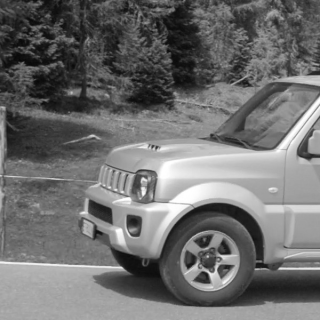
\includegraphics[width=0.9\textwidth]{one_gray.png}
%         \caption{one\_gray.png}
%     \end{subfigure}
%     \begin{subfigure}{0.32\textwidth}
%         \centering
%         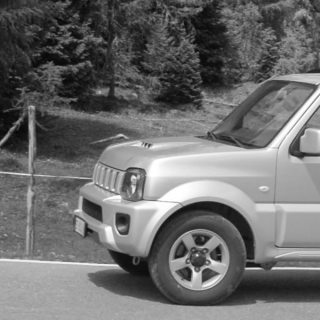
\includegraphics[width=0.9\textwidth]{two_gray.png}
%         \caption{two\_gray.png}
%     \end{subfigure}
%     \caption{Original frames}
% \end{figure}

\section*{Run length encoding and decoding}

The result image is showing below:

\begin{figure}[H]
    \centering
    \begin{subfigure}{0.32\textwidth}
        \centering
        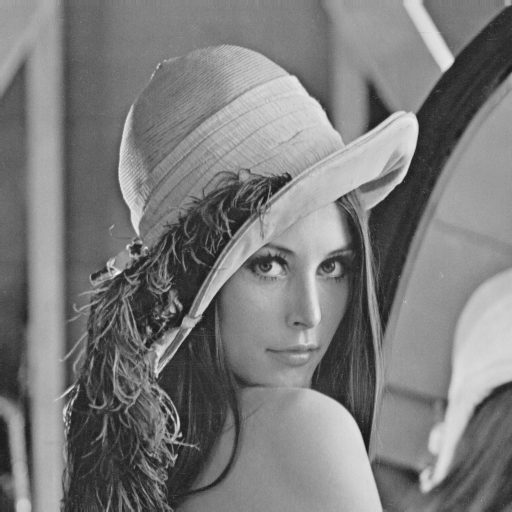
\includegraphics[width=0.9\textwidth]{original_image.png}
        \caption{Original image}
    \end{subfigure}
    \begin{subfigure}{0.32\textwidth}
        \centering
        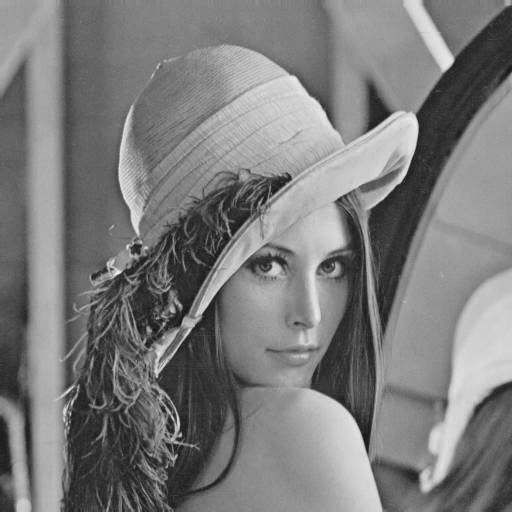
\includegraphics[width=0.9\textwidth]{reconstructed_image_Q1.png}
        \caption{Q1 reconstructed image}
    \end{subfigure}
    \begin{subfigure}{0.32\textwidth}
        \centering
        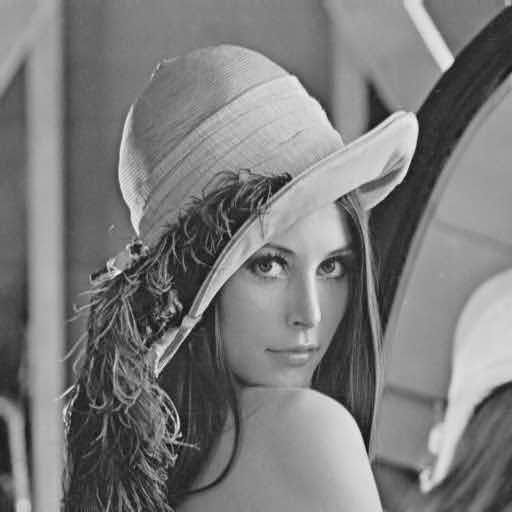
\includegraphics[width=0.9\textwidth]{reconstructed_image_Q2.png}
        \caption{Q2 reconstructed image}
    \end{subfigure}
    \caption{Run length encoding and decoding}
\end{figure}

The encoded image size is shown below:

\begin{table}[H]
    \centering
    \begin{tabular}{|c|c|c|c|}
        \hline
        & Original & Q1 & Q2 \\
        \hline
        Image size (bytes) & 262144 & 79342 & 44582 \\
        \hline
    \end{tabular}
\end{table}

% Original image size: 262144
% Q1 size: 79342 coefficients
% Q2 size: 44582 coefficients

\end{document}